% Toolbar icon: level-set split (MMG) — a domain crossed by an isoline that
% becomes an explicit boundary; the negative side is shaded.
\documentclass[tikz,border=2mm]{standalone}
\usetikzlibrary{arrows.meta,calc,shapes.geometric}
\begin{document}
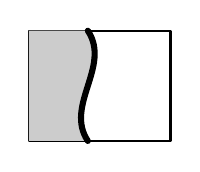
\begin{tikzpicture}[line width=1.3pt, line cap=round, line join=round, x=1mm,y=1mm]
  % domain outline
  \draw[thick] (-9,-7) rectangle (9,7);
  % shaded negative side (left of the isoline)
  \fill[gray!40] (-9,-7) -- (-1.5,-7)
    .. controls (-4.5,-2.5) and (1.5,2.5) .. (-1.5,7)
    -- (-9,7) -- cycle;
  % the isoline itself (the interface the level-set makes explicit)
  \draw[line width=2.2pt] (-1.5,-7)
    .. controls (-4.5,-2.5) and (1.5,2.5) .. (-1.5,7);
\end{tikzpicture}
\end{document}
